\chapter{Wprowadzenie teoretyczne}

\section{Wprowadzenie}
Jako, że problem nie jest powszechnie znany, należy wprowadzić następujące pojęcia \cite{theoryWCRDF}:

\newtheorem{definition}{Definicja}

\begin{definition}
    Funkcja dominująca rzymska zdefiniowana jest dla grafu $G = (V, E)$, gdzie $f: V -> \{0,1,2\}$ spełnia warunek, że dla każdego wierzchołka $u$, dla którego $f(u) = 0$ jest sąsiadem przynajmniej jednego wierzchołka $v$, dla którego $f(v) = 2$.
\end{definition}

\begin{definition}
    Dominujący zbiór $D \subseteq V$ jest zbiorem dominującym słabospójnym grafu $G$ jeśli graf $(V,E \cap (D \times V))$ jest spójny.
\end{definition}

\begin{definition}
    Funkcja dominująca rzymska słabospójna na grafie $G$ będzie funkcją dominującą rzymską, taką, że zbiór $\{u \in V: f(u) \in \{1,2\}\}$ jest jednocześnie zbiorem dominującym słabospójnym.
\end{definition}

\begin{definition}
    Wagę funkcji dominującej rzymskiej słabospójnej definiujemy jako $f(V) = \sum_{u \in V}{f(u)}$. Minimalną wartość tej funkcji nazywamy liczbą dominowania rzymskiego słabospójnego. 
\end{definition}

\begin{figure}[H]
    \centering
    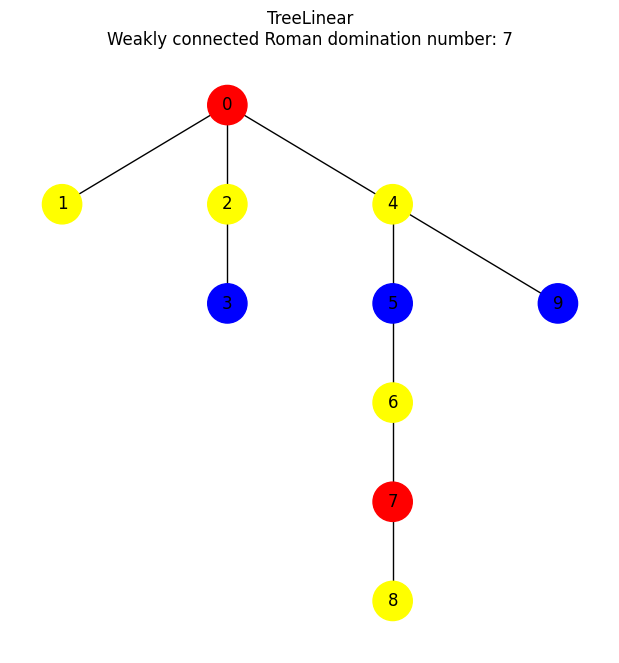
\includegraphics[width=0.5\textwidth]{assets/phase2.png}
    \caption{Przykład grafu rzymskiego słabo spójnego.}
    \label{fig:przykladWCRDF}
\end{figure}

\section{Geneza historyczna}
Problem swoją nazwę zawdzięcza imperium rzymskiemu. Po raz pierwszy został opisany w artykule ,,Defend Roman Empire!".
%tu cytat jeśli znajde w necie
Obrazuje on problem następująco: Każdy wierzchołek grafu reprezentuje pewną lokalizację (miasto, wzgórze) w Imperium Rzymskim. Lokalizacja (wierzchołek $v$) jest niechroniona, jeśli nie stacjonują w niej żadne legiony wojska ($f(v) = 0$) oraz chroniona jeśli ($f(v) \in {1,2} $). Wartości te oznaczają liczbę legionów stacjonujących w danej lokalizacji. Niechroniona lokalizacja może być ochroniona poprzez wysłanie legionu stacjonującego w lokalizacji sąsiadującej. W czwartym wieku cesarz Konstantyn Wielki wydał dekret zakazujący przemieszczenia się legionu do lokalizacji sąsiadującej, jeśli sprawi to, że aktualna lokalizacja pozostanie niechroniona. Dlatego, żeby móc wysłać legion do sąsiedniej lokacji, w aktualnej muszą stacjonować dwa legiony. Oczywiście, cesarzowi zależało na jak najmniejszych kosztach utrzymywania legionów, a zatem, żeby było ich jak najmniej. \cite{theoryWCRDF}

\section{Przegląd literatury}
Omówienie istniejących metod i podejść z literatury, które odnoszą się do problemu badawczego. Jednym z istotnych źródeł w tym zakresie jest strona National Center of Biotechnology Information, która dostarcza bogatych danych do analiz \cite{openai2024}.

\section{Metody badań}
W celu implementacji i testowania wydajności oraz poprawności algorytmów, stworzono program w języku Python, ze wsparciem następujących bibliotek:
\begin{itemize}
    \item networkx - pakiet dostarczający funkcje umożliwiające operacje na grafach, wykresach i sieciach
    \item matplotlib - do wyświetlania wyników działania algorytmów w postaci wykresów grafów
    \item time - wykorzystywane do pomiarów czasu pracy algorytmów
    \item pulp - do programowania liniowego
    \item gurobipy - do programowania liniowego
\end{itemize}

Program umożliwia wprowadzenie dowolnego grafu w postaci listy wierzchołków oraz krawędzi, jak i wygenerowanie losowego grafu. Następnie wybrane algorytmy analizują dany graf poprzez przypisywanie odpowiednich wartości wierzchołkom oraz wyliczania liczby dominowania rzymskiego słabospójnego. Dla każdego z algorytmów wyliczany i zapisywany jest ich czas działania. Na końcu program wyświetla wykres z nadanymi wartościami na wierzchołkach. 

% Opis zastosowanych narzędzi i metod badawczych, w tym szczegóły dotyczące implementacji algorytmów i narzędzi. Zastosowano podejście symulacyjne z wykorzystaniem wytycznych opartych na literaturze \cite{kowalski2002}.

% \section{Wyniki}
% Przedstawienie wyników uzyskanych w trakcie badań, w tym analiza ich dokładności i efektywności \cite{openai2024}.
